The overall process took inspiration from agile software development with a
touch of 'design-school'. \todo{Fix this section.}

\begin{figure}[h!]
  \centering
  \includegraphics{figures/method.pdf}
  \caption{Concept, development, testing and improvement cycle.}
\end{figure}

\section{Brainstorming-sessions and interviews}{\label{label_sectionIdeas}

  In order to figure out a interesting approach, two brainstorming-sessions
  were conducted. The first in order to figure out what could be beneficial
  to the team and studio at large. Secondly, discussing possible academic
  applications and results.

  After hearing about the communication regression, it was decided that
  it would be interesting to see if there are certain design elements and
  theories that hold up better under stressful scenarios than others. A
  secondary goal included trying to make a testing platform 'from-scratch'
  in order to see if it would be feasible for a smaller research- or
  developer-team to conduct similar evaluations in-house on a small budget.

  To deicide what type of mock-assignments the tests should be constructed
  from, three in-person interviews were conducted. The managers were asked
  about what they would like to see implemented in order to make their
  day-to-day work easier, producing the following ideas:

  \newcommand{\ideaOne}{%
    An easy way to see if a co-worker is assigned more work than they have
    available hours.%
  }

  \newcommand{\ideaTwo}{%
    Calendar overview where it is possible to determine if there are
    hot-spots where lots of results need to be produced at the same
    time.%
  }

  \newcommand{\ideaThree}{%
    A concise way to identify if there are critical tasks that, if
    delayed, would delay other tasks that depend on it.%
  }

  \newcommand{\ideaFour}{%
    The possibility to identify a group or teams strengths and assign
    task types accordingly.%
  }

  \begin{itemize}
    \item{\ideaOne\label{label_ideas}}
    \item{\ideaTwo}
    \item{\ideaThree}
    \item{\ideaFour}
  \end{itemize}


\section{Lo-fi prototypes}

  After taking some pointers from \findref, together with the suggestions
  gathered from the manager-interviews, four simple paper prototypes, shown
  below, were printed and presented to a second group of five interviewees
  for evaluation.

    \begin{figure}[h!]
      \center
      \includegraphics[valign=t,trim={.10cm .10cm .35cm .25cm},clip,width=.49\linewidth]{ui11.pdf}
      \includegraphics[valign=t,trim={.15cm .30cm .20cm .20cm},clip,width=.49\linewidth]{ui12.pdf}
      \includegraphics[valign=t,trim={.45cm .55cm .65cm .35cm},clip,width=.49\linewidth]{ui13.pdf}
      \includegraphics[valign=t,trim={.25cm .35cm .30cm .25cm},clip,width=.49\linewidth]{ui14.pdf}
      \caption{Interface drafts 1.1, 1.2, 1.3 and 1.4}
      \label{label_mockupInterfaces}
    \end{figure}

  The main difference is the placement of the main interface elements, with
  the first group having them on top, and the second one the left side.
  Lager versions of prototypes and itemized result from the interviews are
  found in \todoInsert{result link for interviews and larger prototypes.}

  \subsection{Interview structure for prototype selection}

    \begin{figure}[h!]
      \centering
      \includegraphics[trim={0 0 0 0},clip]{figures/lofi_method.pdf}
      \caption{Overall structure of prototype selection interviews.}
    \end{figure}

    These interviews were conducted in-person, with five team members, on
    the premises of Massive. The interview started with a description of
    what was happening; an evaluation of four different mock-up interfaces
    to determine which one was the most suitable for further testing.

    After confirming that there were no immediate questions, the
    interviewee was presented with the printed mockups in the same
    arrangement as shown in figure \ref{label_mockupInterfaces}. They were
    then asked to evaluate, out loud, the interfaces in any order they
    wished, and to ask if there was anything unclear about the assumed
    functionality.

    When the participant felt they were done and any questions they had
    about the interface were sorted out, they were asked to sort the
    prototypes from best- to least-suited for the upcoming test purpose.
    Again, the participant was asked to voice their thought process out
    aloud as they did the sorting.

    After confirming that the interviewee was satisfied with their
    ordering, a set of ten flash-cards were introduced. These cards
    represent the combined key-words-attributes from ISO 9241-11{\findref}
    and ISO 9241-12{\findref}, concerning usability and presentation of
    information respectively.

    Keyword definitions presented below:

        \begin{description}[style=nextline]
          \item[Effectiveness]{
            Usability is measured by the extend to which the
            intended goals of use of the overall system are achieved.
          }
          \item[Efficiency]{
            The resources that have to be expended to achieved the indented
            goals.
          }
          \item[Satisfaction]{
            The extent to which the user finds the overall system
            acceptable.
          }
          \item[Clarity]{
              The information content is conveyed quickly and accurately.
          }
          \item[Discriminability]{
              The displayed information can be distinguished
              accurately.
          }
          \item[Conciseness]{
              Users are not overloaded with extraneous information.
          }
          \item[Consistency]{
              A unique design, conformity with user's expectation.
          }
          \item[Detectability]{
              The user's attention is directed towards information
              required.
          }
          \item[Legibility]{
              Information is easy to read.
          }
          \item[Comprehensibility]{
              The maning is clearly understandable, unambiguous,
              interpretable, and recognizable.
          }
        \end{description}

    Where the top three terms are defined in ISO 9241-11 with the remainder
    coming from ISO 9241-12.

    The next task was for each participant to order the keywords
    in order of how important they thought that specific quality was for a
    well-functioning, user interfacing software. There were no restrictions
    in regards to the number of times a participant could ask about the
    definition or clarification of each term.

    When the participant acknowledged that they were finished with their
    selection, it was recorded, and the were asked to do one final task.
    Each participant was asked to re-evaluate their previously selected
    ranking of the prototype interfaces, changing the order if they felt
    another one was more appropriate after being exposed to the ISO
    definitions.

%        evaluation. The evaluation was conducted as an in-person interview
%        where the interviewee was asked to voiced their thoughts out aloud.
%        After the initial reaction and thought about each of the designs, the
%        interviewee was asked to pick, according to them, the most suitable
%        design.
%
%        After the initial pick, the interviewee was presented with
%        \todoInsert{part about ISO-standard design}, which they had to arrange
%        in order of most to least important according to their own views.
%        After prioritizing the different design attributes, the participant was
%        again asked to pick what they felt was the most suitable design.
%
%
%        \todo{Expand with information about ISO design standard}
%

\section{Hi-fi prototype}

After completing the interviews and tallying which paper prototype that
was sorted first the most times, the result was paper prototype 1.4.

\begin{figure}[h!]
  \centering
  \includegraphics{figures/test_flow.pdf}
  \caption{Illustrated flow for overall test-session.}
\end{figure}

\begin{figure}[h!]
  \centering
  \includegraphics{figures/test_flow_task_runs.pdf}
  \caption{Illustrated flow for individual task-runs.}
\end{figure}


  \subsection{Input methods and screen sizes}

  \todo{Spell out the input alternatives} While the choices for the input
  method, except the last one, corresponds directly to a concrete input
  method used in human-computer interactions, the screen-sizes are somewhat
  ambiguous. This was an active choice in order to not alienate
  participants by forcing them to specify an actual measurement for the
  screen size. The assumed values for the screen-sizes ranges for the given
  choices are:
  \textit{Desktop} $>$17",
  \textit{Laptop}  12"-17",
  \textit{Tablet}  7"-12" and
  \textit{Mobile}  $<$7".

  \subsection{General information, consent and initial survey}

  When accessing the test the participant is greeted by a information and
  consent screen, detailing the goals of the test and how the information
  generated by their activity will be used. The page explains that this
  is a usability study, and though there will be information collected,
  anything that will be publicised will be aggregations and include no
  personally identifiable information. The full information and consent
  page can be found in figure \ref{label_infoConsent}.

  Participant that accept and submit the consent form are then navigated
  to the main landing page. This page acts as a hub for the duration of
  the test session, providing access to all other parts of testing
  application. On the first visit the main view of the landing page is
  occupied by the initial survey, shown below.

  \begin{figure}[h!]
    \centering
    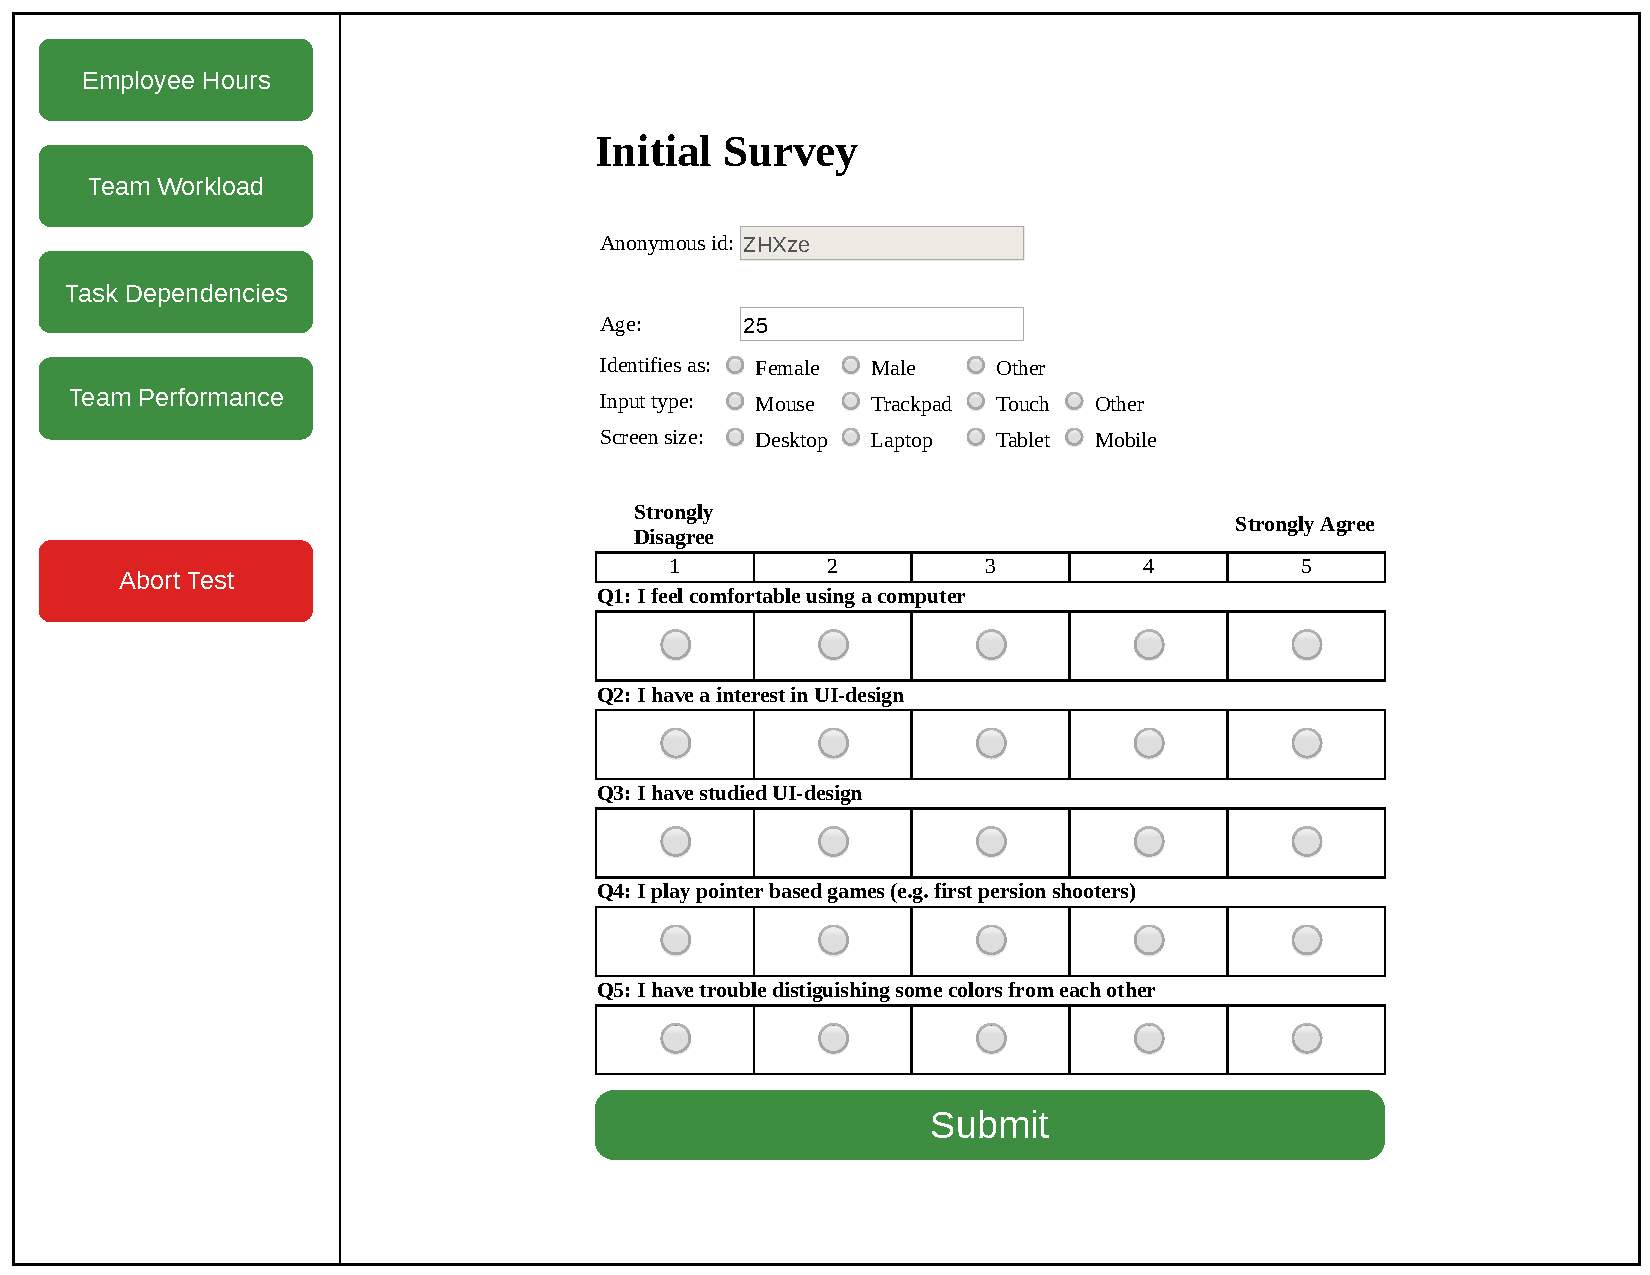
\includegraphics[width=.7\textwidth]{figures/captures/webapp_pre_survey.pdf}
    \caption{Capture of initial survey page.}
    \label{label_preSurvey}
  \end{figure}

  While it is possible for the participant to interact with the buttons on
  the left side before the initial survey is submitted, pressing any of the
  buttons except 'Abort Test' will only display the same survey-page.

  \begin{figure}[h!]
    \centering
    \fbox{
      \includegraphics[trim={4cm 8cm 9cm 8cm},clip,width=.5\textwidth]{figures/captures/webapp_abort.pdf}
    }
    \caption{Capture of confirmation page for aborting the test.}
    \label{label_abort}
  \end{figure}

  The dedicated 'Abort Test' button is available in all the different
  views of the application, in case the participant no longer wants to
  participate for any reason. Pressing this button displays a page
  explaining that continuing will scrub any activity related to their
  current anonymous id from the database and abort the current test.
  %Additionally and return it to the pool
  %of available identification strings.


  \subsection{Landing page}

  After the participant has submitted the pre-survey, it  disappears and is
  replaced by a few basic statistics about the current test session.
  The functionality of the left-side buttons is restored and makes it
  possible to choose any of the following four test types:
  \textit{Employee Hours},
  \textit{Team Workload},
  \textit{Task Dependencies} and
  \textit{Team Performance}.

  \begin{figure}[h!]
    \centering
    \includegraphics[width=.7\textwidth]{figures/captures/webapp_main_statistics.pdf}
    \caption{Capture of the hub page, post initial survey, default state.}
    \label{label_mainStatistics}
  \end{figure}

  The session-statistics include the participants assigned anonymous id,
  how many test of each type they have completed and how many test they
  have to complete in order for the post-survey to become available.

  Requiring five tests before making the post-survey available is the only
  hard limitation placed on the participants. Other than the test-minimum
  there is no limit on how many tests they can perform or how long time
  they take to complete a individual test or the test session as a whole.

  \subsection{Information, fictional context and execution}

  Before starting any of the tasks, the participant is greeted by a page
  containing the general information about the task at hand. Each of the
  pages follows the same structure with three sections, \textit{Goal},
  \textit{How} and \textit{Summary}, explained below.
  \todo{Re-edit}

  The \textit{Goal} section should be short{\findref}, a sentence at
  most{\findref}, and tell the participant what they need to do in order
  to complete the task successfully.

  After reading the \textit{How} section, the participant should have a
  basic understanding of how the information related to the test is
  structured and presented. If there are any specific details about the
  representation of the task that are deemed essential they should be
  described in this section.

  The \textit{Summary} section is meant to repeat the information in the
  \textit{How} section, but in a different and briefer fashion in order
  to help with retention\findref.

  Lastly, the participant is told that the same information that has just
  been presented is available after starting the test, accessible by
  hovering the cursor over a '?' in the upper left corner.

  Since all the task-mechanics boil down to
  \textit{find the element and press it as fast as possible},
  the intent is to give the participant enough concrete
  information about the test at hand while trying to maintain the
  implied fictional context of the task. Which means the tone of any
  instructions or information should be closer to
  \textit{''select the co-worker with the most X''} rather than
  \textit{''click the largest box''}.
  \todoMaybe{Colorswatches}
  \todoMaybe{Range of values}
  \todoMaybe{Randomization-1 + max}
  \todoMaybe{Add about no feedback on result -> BAD}

%pallet = [
%  "#001f3f",
%  "#0074D9",
%  "#39CCCC",
%  "#3D9970",
%  "#2ECC40",
%  "#01FF70",
%  "#FFDC00",
%  "#FF851B",
%  "#85144b",
%  "#F012BE",
%  "#B10DC9"
%]

%      \subsection{Task - employee hours}
  \subsection{Employee hours}

    \textit{\ideaOne}

    The premise for this task is that the organization generating the data
    utilizes some form of task assigning system together with a
    cost-estimation system. In short, there is a set of tasks that need to
    be done, each with a estimated time-cost, and a number of people that
    can be scheduled to do said work.

    Given there is a limited amount of time that any assignee can spend
    working, it is possible to over-schedule someone. In this scenario,
    being over-scheduled is the result of having more work scheduled to you
    over a period of time than the total available capacity for the same
    period. In summary, the goal of this task consists of identifying these
    cases, in particular, the person that is the most over-scheduled.

    \begin{figure}[h!]
      \centering
      \includegraphics[width=.49\textwidth]{figures/captures/webapp_employee_hours_info.pdf}
      \includegraphics[width=.49\textwidth]{figures/captures/webapp_employee_hours_task.pdf}
      \caption{Capture of Employee Hours information and task page.}
    \end{figure}

    After starting the task, the participant is shown a bar-graph with bars
    of varying heights and coloring. Each bar shows the relation between
    available and scheduled work-time for one out of the twenty-five
    represented people.

    Here, the height of the black outline of each bar represents the
    \textit{available work-capacity}, the varying heights simulating the
    difference of available hours due to to sick-leave, vacations or
    different contracts.

    The \textit{total scheduled workload} for
    each person is represented by the height of the colored segments in
    each bar. If there is capacity left the colored segment will not extend to the
    top of the bar outline, leaving a white segment representing
    non-scheduled time. On the other hand, if the amount of scheduled work
    is greater than the available capacity, the color will extend beyond
    the original outline and be colored differently for readability.

    In summary, the height of a white segments in a bar represent the
    amount of remaining capacity, while the height of any other-colored
    segment signifies how \textit{over-scheduled} someone is. Find the
    largest other-colored segment it and click on it.

%      \subsection{Task - team workload}
  \subsection{Team workload}

    \textit{\ideaTwo}

    In the following scenario the business or organization has a schedule,
    Monday to Friday, that stretches twenty-five weeks into the future. The
    goal is to keep the workload as steady as possible without to many
    jumps in either direction. Have to little to do and people are
    underutilized and in worst case, bored. Have to much that needs to be
    done at the same time and people might burn out. Avoiding both
    extremes would be preferable.

    \begin{figure}[h!]
      \centering
      \includegraphics[width=.49\textwidth]{figures/captures/webapp_team_workload_info.pdf}
      \includegraphics[width=.49\textwidth]{figures/captures/webapp_team_workload_task.pdf}
      \caption{Capture of Team Workload information and task page.}
    \end{figure}

    Running this test shows the participant a grid of twenty-five rows
    consisting of five columns each, denoted
    \texttt{MON},
    \texttt{TUE},
    \texttt{WED},
    \texttt{THU} and
    \texttt{FRI},
    representing the scheduled twenty-five workweeks mentioned above. Each
    of the rectangles are colored with the same color but differ in the
    saturation. A cell that has zero saturation, or white in this case,
    signal that no work is scheduled for completion on that particular day.
    Inversely, the darker a cell is, the more work needs to be completed on
    that specific day.

    Since there needs to be a clearly defined goal for each test, there has
    to be a choice between bored and burned out people, where the latter
    seems far worse. Now the problem can be corrected by identifying days
    where there is an extra high amount of work that needs to be done, and
    try to re-schedule it to less busy days.

    For the participant executing the test, the goal is to find the
    darkest, or most saturated rectangle and click it as fast as possible.

  \subsection{Task dependencies}

    \textit{\ideaThree}

    The assumption for this test is that the underlying system producing
    the data has tasks that need to be completed first in order for other
    tasks to complete in turn, in short, dependencies. This test revolves
    around answering the question
    \textit{''which elements are the most crucial for the overall
      process?''}. The answer to this question can be very useful, as an
    example, when being forced to cut back on things due to limited
    resources while trying to affect as few other things as possible.

    \begin{figure}[h!]
      \centering
      \includegraphics[width=.49\textwidth]{figures/captures/webapp_dependencies_info.pdf}
      \includegraphics[width=.49\textwidth]{figures/captures/webapp_dependencies_task.pdf}
      \caption{Capture of Task Dependencies info- and task-page.}
    \end{figure}

    Initializing this test shows the participant seventeen small circles,
    representing tasks, arranged in a larger circle. Additionally, there are
    colored lines connecting some circles together, indicating there is
    a dependency between them, more lines equals more dependencies.

    Since the stated interest in knowing how dependent the different
    moving parts are on each other, knowing which task has the most
    dependencies is a good start. In terms of what the participant has to
    do to finish the test, this translates to; find the task with the most
    connections and click on it as fast as possible.

   % \subsection{Task - team performance}
    \subsection{Team performance}

    \textit{\ideaFour}

    Given a working-environment where things are done in parallell it
    becomes interesting to know if a specific group or individual is
    especially effective in a certain area. Having this information makes
    it possible to assign people, if they excel at a specific area, to
    tasks that match their abilities.

    In this test there are five different task-categories,
    \textit{tickets},
    \textit{rnd},
    \textit{support},
    \textit{features} and
    \textit{maintentance}.

    \begin{figure}[h!]
      \centering
      \includegraphics[width=.49\textwidth]{figures/captures/webapp_team_performance_info.pdf}
      \includegraphics[width=.49\textwidth]{figures/captures/webapp_team_performance_task.pdf}
      \caption{Capture of Team Performance info- and task-page.}
    \end{figure}

    This task presents the participant with bars showcasing the total
    completed work-load for nine different teams over an unspecified amount
    of time.

    There are two types of information shown, the total amount of work done
    by each team, represented by the total horizontal length of the bar.
    And the amount of the total work that went into a specific
    task-section, represented by the length of each individual sub-section
    of the overall bar.
    In order to correctly answer this test, the participant first needs to
    identify which of the bars is the longest one, and then identify which
    sub-section is the largest one, and click on that one.

  \subsection{Post survey}

    As the participant completes five or more tests the 'Take Survey'
    button becomes active, pressing this button sends the participant to
    the post-survey page. Other than the survey itself, there is also the
    option to return to the tests if the button was pressed by accident or
    if the participant had a change of mind.

    The post-survey consist of eight questions and an optional input field
    for additional comments. These questions are ment to evaluate the
    participants thoughts about the current iteration of the testing
    application in order to derive possible improvement for the next
    implementation iteration.

    Options that are of interest include, among others, if the goal of each
    task was clear, if the application was pleasing to look at, if the use of
    colors help when navigating application, etcetera. For a verbatim list of
    the questions used in the post-questionnaire see figure
    \todoInsert{reference to post-survey}.

